\section{Experiments}
\subsection{Implementation Details.}
We trained Mono3DV on a single NVIDIA 3090 GPU for 250 epochs. We used a batch size of 8 and an initial learning rate of $2 \times 10^{-4}$. Further training specifics are detailed in ~\Cref{tab:hyper}.

\begin{table}[h!]
    \centering
    \caption{\textbf{Main hyperparameters of Mono3DV on KITTI Dataset.}}
    \begin{tabular}{ll}
         \toprule
         \textbf{Item} & \textbf{Value} \\
         \midrule
         $\lambda_1$ & 1  \\
         $\lambda_2$ & 1 \\
         $\lambda_3$ & 0.5 \\
         $\lambda_C$ & 0.4 \\
         $\lambda_D$ & 0.2 \\
         $\epsilon$ & 1 \\
         $T$ & 85 \\
         $N$ & 50 \\
         $G$ & 11\\
         $C$ & 5 \\
         $\beta$ & 4\\
         weight decay & 1e-4\\
         scheduler & Step \\
         decay rate & 0.5 \\
         decay list & [85, 125, 165, 205] \\
         number of feature scales & 4 \\
         hidden dim & 256 \\
         feedforward dim & 256 \\
         dropout & 0.1 \\
         nheads & 8 \\
        number of encoder layers & 3 \\
        number of decoder layers & 3 \\
         encoder npoints  & 4 \\
         decoder points & 4\\
         \bottomrule
    \end{tabular}
    \label{tab:hyper}
\end{table}

\subsection{Main Results}
\label{sec:mono3dv:main_results}

\begin{table*}[h!]
\centering
\caption{Comparisons with state-of-the-art monocular methods on the KITTI test and val sets for the car category. We \textbf{bold} the best results and \underline{underline} the second-best results. The {\color[HTML]{3166FF} blue} refers to the gain and the {\color[HTML]{FE0000} red} is the decrease of our method.}
\resizebox{\textwidth}{!}{%\textbf{
\begin{tabular}{l|c|c|clcc|ccc|clcc|clcc}
\hline
\multicolumn{1}{c|}{} & & & \multicolumn{4}{c|}{Test, $AP_{3D|R40}$} & \multicolumn{3}{c|}{Test, $AP_{BEV|R40}$} & \multicolumn{4}{c|}{Val, $AP_{3D|R40}$} & \multicolumn{4}{c}{Val, $AP_{BEV|R40}$} \\ \cline{4-18}
\multicolumn{1}{l|}{\multirow{-2}{*}{Methods}} & \multirow{-2}{*}{Extra data} & \multirow{-2}{*}{Reference} & \multicolumn{2}{c}{Easy} & Mod. & Hard & Easy & Mod. & Hard & \multicolumn{2}{c}{Easy} & Mod. & Hard & \multicolumn{2}{c}{Easy} & Mod. & Hard \\ \hline
MonoDTR~\cite{MonoDTR} & & CVPR 2022 & \multicolumn{2}{c}{21.99} & 15.39 & 12.73 & 28.59 & 20.38 & 17.14 & \multicolumn{2}{c}{24.52} & 18.57 & 15.51 & \multicolumn{2}{c}{33.33} & 25.35 & 21.68 \\
DID-M3D~\cite{DID-M3D} &  & ECCV 2022 & \multicolumn{2}{c}{24.40} & 16.29 & 13.75 & 32.95 & 22.76 & 19.83 & \multicolumn{2}{c}{22.98} & 16.12 & 14.03 & \multicolumn{2}{c}{31.10} & 22.76 & 19.50 \\
OccupancyM3D~\cite{OccupanyM3D} & \multirow{-3}{*}{LiDAR} & CVPR 2024 & \multicolumn{2}{c}{25.55} & 17.02 & 14.79 & \underline{35.38} & 24.18 & \underline{21.37} & \multicolumn{2}{c}{26.87} & 19.96 & 17.15 & \multicolumn{2}{c}{35.72} & 26.60 & 23.68 \\ \hline
MonoPGC~\cite{MonoPGC} &  & ICRA 2023 & \multicolumn{2}{c}{24.68} & 17.17 & 14.14 & 32.50 & 23.14 & 20.30 & \multicolumn{2}{c}{25.67} & 18.63 & 15.65 & \multicolumn{2}{c}{34.06} & 24.26 & 20.78 \\
OPA-3D~\cite{OPA-3D} & \multirow{-2}{*}{Depth} & RAL 2023 & \multicolumn{2}{c}{24.60} & 17.05 & 14.25 & 33.54 & 22.53 & 19.22 & \multicolumn{2}{c}{24.97} & 19.40 & 16.59 & \multicolumn{2}{c}{33.80} & 25.51 & 22.13 \\ \hline
MonoCon~\cite{MonoCon} &  & AAAI 2022 & \multicolumn{2}{c}{22.50} & 16.46 & 13.95 & 31.12 & 22.10 & 19.00 & \multicolumn{2}{c}{26.33} & 19.01 & 15.98 & \multicolumn{2}{c}{-} & - & - \\
DEVIANT~\cite{DEVIANT} &  & ECCV 2022 & \multicolumn{2}{c}{21.88} & 14.46 & 11.89 & 29.65 & 20.44 & 17.43 & \multicolumn{2}{c}{24.63} & 16.54 & 14.52 & \multicolumn{2}{c}{32.60} & 23.04 & 19.99 \\
MonoDDE~\cite{MonoDDE} &  & CVPR 2022 & \multicolumn{2}{c}{24.93} & 17.14 & 15.10 & 33.58 & 23.46 & 20.37 & \multicolumn{2}{c}{26.66} & 19.75 & 16.72 & \multicolumn{2}{c}{35.51} & 26.48 & 23.07 \\
MonoUNI~\cite{MonoUNI} &  & NeurlPS 2023 & \multicolumn{2}{c}{24.75} & 16.73 & 13.49 & - & - & - & \multicolumn{2}{c}{24.51} & 17.18 & 14.01 & \multicolumn{2}{c}{-} & - & - \\
MonoDETR~\cite{MonoDETR} &  & ICCV 2023 & \multicolumn{2}{c}{25.00} & 16.47 & 13.58 & 33.60 & 22.11 & 18.60 & \multicolumn{2}{c}{28.84} & 20.61 & 16.38 & \multicolumn{2}{c}{37.86} & 26.95 & 22.80 \\
MonoCD~\cite{MonoCD} &  & CVPR 2024 & \multicolumn{2}{c}{25.53} & 16.59 & 14.53 & 33.41 & 22.81 & 19.57 & \multicolumn{2}{c}{26.45} & 19.37 & 16.38 & \multicolumn{2}{c}{34.60} & 24.96 & 21.51 \\
FD3D~\cite{FD3D} & & AAAI 2024 & \multicolumn{2}{c}{25.38} & 17.12 & 14.50 & 34.20 & 23.72 & 20.76 & \multicolumn{2}{c}{28.22} & 20.23 & 17.04 & \multicolumn{2}{c}{36.98} & 26.77 & 23.16 \\
MonoDGP~\cite{MonoDGP} & \multirow{-8}{*}{None} & CVPR 2025 & \multicolumn{2}{c}{\underline{26.35}} & \underline{18.72} & \underline{15.97} & 35.24 & \textbf{25.23} & \textbf{22.02} & \multicolumn{2}{c}{\underline{30.76}} & \underline{22.34} & \underline{19.02} & \multicolumn{2}{c}{\underline{39.40}} & \underline{28.20} & \underline{24.42} \\ \hline
Mono3DV (Ours) & None & - & \multicolumn{2}{c}{\textbf{28.26}} & \textbf{19.20} & \textbf{16.21} & \textbf{35.77} & \underline{24.82} & \underline{21.37} & \multicolumn{2}{c}{\textbf{32.12}} & \textbf{23.55} & \textbf{20.15} & \multicolumn{2}{c}{\textbf{40.85}} & \textbf{29.24} & \textbf{25.49} \\
Improvement & - & - & \multicolumn{2}{c}{{\color[HTML]{3166FF} +1.91}} & {\color[HTML]{3166FF} +0.48} & {\color[HTML]{3166FF} +0.24} & {\color[HTML]{3166FF} +0.39} & {\color[HTML]{FE0000} -0.41} & {\color[HTML]{FE0000} -0.65} & \multicolumn{2}{c}{{\color[HTML]{3166FF} +1.36}} & {\color[HTML]{3166FF} +1.21} & {\color[HTML]{3166FF} +1.13} & \multicolumn{2}{c}{{\color[HTML]{3166FF} +1.45}} & {\color[HTML]{3166FF} +1.04} & {\color[HTML]{3166FF} +1.07} \\ \hline
\end{tabular}}
\label{tab:mono3dv_main_result}
\end{table*}

\noindent\textbf{Experiment on the KITTI 3D test set.}
As shown in \Cref{tab:mono3dv_main_result}, our Mono3DV method demonstrates superior performance on the KITTI test set compared to state-of-the-art monocular 3D object detection methods. Specifically, Mono3DV achieves a significant improvement in $\mathbf{AP_{3D}}$, surpassing the second-best method by $+1.91\%$, $+0.48\%$, and $+0.24\%$ across the three difficulty levels. Furthermore, it outperforms the second-best in $\mathbf{AP_{BEV}}$ by $0.39\%$ under the easy difficulty while maintaining competitive performance for moderate and hard cases. These results underscore the effectiveness of our proposed framework for accurate 3D object prediction from monocular images.

\noindent\textbf{Experiment on the KITTI 3D val set.} We also evaluated our approach on the KITTI validation dataset. As presented in \Cref{tab:mono3dv_main_result}, our Mono3DV demonstrates superior performance compared to all existing methods. Notably, it surpasses the second-best approach under three-level difficulties by $+1.36\%$, $+1.21\%$, and $+1.13\%$ in $\mathbf{AP_{3D}}$, and by $+1.45\%$, $+1.04\%$, and $+1.07\%$ in $\mathbf{AP_{BEV}}$. These results further emphasize the effectiveness of Mono3DV.

\noindent\textbf{Experiment on the Waymo Open Dataset.} As detailed in~\Cref{tab:waymo_experiment}, Mono3DV delivers state-of-the-art results at every distance range without the need for additional training data. Its exceptional performance on distant objects, in particular, highlights the method's overall effectiveness and strong generalization capabilities.
\begin{table*}[!ht]
\centering
\caption{Results on the Waymo val set for the vehicle category. Compared with methods without extra data, we \textbf{bold} the best results and \underline{underline} the second-best results.}
\resizebox{\columnwidth}{!}{%
\begin{tabular}{c|l|c|cccc|cccc}
\hline
\multirow{2}{*}{Difficulty} & \multirow{2}{*}{Methods} & \multirow{2}{*}{Extra} & \multicolumn{4}{c|}{$AP_{3D}$} & \multicolumn{4}{c}{$APH_{3D}$} \\ 
\cline{4-11} 
 &  &  & All & 0-30 & 30-50 & 50-$\infty$ & All & 0-30 & 30-50 & 50-$\infty$ \\ 
\hline
\multirow{8}{*}{{Level\_1 \newline (IoU=0.7)}} 
 & PatchNet \cite{patchnet} in \cite{pct} & Depth & 0.39 & 1.67 & 0.13 & 0.03 & 0.39 & 1.63 & 0.12 & 0.03 \\
 & PCT \cite{pct} & Depth & 0.89 & 3.18 & 0.27 & 0.07 & 0.88 & 3.15 & 0.27 & 0.07 \\
 & M3D-RPN \cite{m3d-rpn} in \cite{CaDDN} & None & 0.35 & 1.12 & 0.18 & 0.02 & 0.34 & 1.10 & 0.18 & 0.02 \\
 & GUPNet \cite{GUPNet} in \cite{DEVIANT} & None & 2.28 & 6.15 & 0.81 & 0.03 & 2.27 & 6.11 & 0.80 & 0.03 \\
 & DEVIANT \cite{DEVIANT} & None & 2.69 & 6.95 & 0.99 & 0.02 & 2.67 & 6.90 & 0.98 & 0.02 \\
 & MonoUNI \cite{MonoUNI} & None & 3.20 & 8.61 & 0.87 & 0.13 & 3.16 & 8.50 & 0.86 & 0.12 \\
 & MonoDGP \cite{MonoDGP} & None & \underline{4.28} & \underline{10.24} & \underline{1.15} & \underline{0.16} & \underline{4.23} & \underline{10.10} & \underline{1.14} & \underline{0.16} \\ 
 & \textbf{Mono3DV (Ours)} & None & \textbf{4.84} & \textbf{11.02} & \textbf{1.28} & \textbf{0.19} & \textbf{4.68} & \textbf{10.78} & \textbf{1.23} & \textbf{0.18} \\
\hline
\multirow{8}{*}{{Level\_2\newline (IoU=0.7)}} 
 & PatchNet \cite{patchnet} in \cite{pct} & Depth & 0.38 & 1.67 & 0.13 & 0.03 & 0.36 & 1.63 & 0.11 & 0.03 \\
 & PCT \cite{pct} & Depth & 0.66 & 3.18 & 0.27 & 0.07 & 0.66 & 3.15 & 0.26 & 0.07 \\
 & M3D-RPN \cite{m3d-rpn} in \cite{CaDDN} & None & 0.35 & 1.12 & 0.18 & 0.02 & 0.33 & 1.10 & 0.17 & 0.02 \\
 & GUPNet \cite{GUPNet} in \cite{DEVIANT} & None & 2.14 & 6.13 & 0.78 & 0.02 & 2.12 & 6.08 & 0.77 & 0.02 \\
 & DEVIANT \cite{DEVIANT} & None & 2.52 & 6.93 & 0.95 & 0.02 & 2.50 & 6.87 & 0.94 & 0.02 \\
 & MonoUNI \cite{MonoUNI} & None & 3.04 & 8.59 & 0.85 & 0.12 & 3.00 & 8.48 & 0.84 & 0.12 \\
 & MonoDGP \cite{MonoDGP} & None & \underline{4.00} & \underline{10.20} & \underline{1.13} & \underline{0.15} & \underline{3.96} & \underline{10.08} & \underline{1.12} & \underline{0.15} \\ 
 & \textbf{Mono3DV (Ours)} & None & \textbf{4.55} & \textbf{10.89} & \textbf{1.31} & \textbf{0.17} & \textbf{4.46} & \textbf{10.68} & \textbf{1.20} & \textbf{0.17} \\
\hline
\multirow{8}{*}{{Level\_1\newline (IoU=0.5)}} 
 & PatchNet \cite{patchnet} in \cite{pct} & Depth & 2.92 & 10.03 & 1.09 & 0.23 & 2.74 & 9.75 & 0.96 & 0.18 \\
 & PCT \cite{pct} & Depth & 4.20 & 14.70 & 1.78 & 0.39 & 4.15 & 14.54 & 1.75 & 0.39 \\
 & M3D-RPN \cite{m3d-rpn} in \cite{CaDDN} & None & 3.79 & 11.14 & 2.16 & 0.26 & 3.63 & 10.70 & 2.09 & 0.21 \\
 & GUPNet \cite{GUPNet} in \cite{DEVIANT} & None & 10.02 & 24.78 & 4.84 & 0.22 & 9.94 & 24.59 & 4.78 & 0.22 \\
 & DEVIANT \cite{DEVIANT} & None & 10.98 & 26.85 & 5.13 & 0.18 & 10.89 & 26.64 & 5.08 & 0.18 \\
 & MonoUNI \cite{MonoUNI} & None & 10.98 & 26.63 & 4.04 & 0.57 & 10.73 & 26.30 & 3.98 & 0.55 \\
 & MonoDGP \cite{MonoDGP} & None & \underline{12.36} & \underline{31.12} & \underline{5.78} & \underline{1.24} & \underline{12.18} & \underline{30.68} & \underline{5.71} & \underline{1.22} \\ 
 & \textbf{Mono3DV (Ours)} & None & \textbf{13.53} & \textbf{34.72} & \textbf{6.11} & \textbf{1.59} & \textbf{13.28} & \textbf{33.81} & \textbf{6.19} & \textbf{1.57} \\
\hline
\multirow{8}{*}{{Level\_2\newline (IoU=0.5)}} 
 & PatchNet \cite{patchnet} in \cite{pct} & Depth & 2.42 & 10.01 & 1.07 & 0.22 & 2.28 & 9.73 & 0.97 & 0.16 \\
 & PCT \cite{pct} & Depth & 4.03 & 14.67 & 1.74 & 0.36 & 4.15 & 14.51 & 1.71 & 0.35 \\
 & M3D-RPN \cite{m3d-rpn} in \cite{CaDDN} & None & 3.61 & 11.12 & 2.12 & 0.24 & 3.46 & 10.67 & 2.04 & 0.20 \\
 & GUPNet \cite{GUPNet} in \cite{DEVIANT} & None & 9.39 & 24.69 & 4.67 & 0.19 & 9.31 & 24.50 & 4.62 & 0.19 \\
 & DEVIANT \cite{DEVIANT} & None & 10.29 & 26.75 & 4.95 & 0.16 & 10.20 & 26.54 & 4.90 & 0.16 \\
 & MonoUNI \cite{MonoUNI} & None & 10.38 & 26.57 & 3.95 & 0.53 & 10.24 & 26.24 & 3.89 & 0.51\\
 & MonoDGP \cite{MonoDGP} & None & \underline{11.71} & \underline{31.02} & \underline{5.61} & \underline{1.17} & \underline{11.56} & \underline{30.58} & \underline{5.54} & \underline{1.15} \\ 
  & \textbf{Mono3DV (Ours)} & None & \textbf{12.92} & \textbf{34.65} & \textbf{5.93} & \textbf{1.48} & \textbf{12.76} & \textbf{34.08} & \textbf{5.87} & \textbf{1.46} \\
\hline 
\end{tabular}}
\label{tab:waymo_experiment}
\end{table*}

\noindent\textbf{Plug-and-play Experiments for Multi-view Detectors.} As shown in~\Cref{tab:nuscence_result}, for RayDN~\cite{RayDN}, our approach delivered +0.8\% NDS and +0.9\% mAP by optimizing learnable query denoising and iterative refinement strategies. Applied to OPEN~\cite{OPEN}, it achieved +1.2\% NDS and +1.1\% mAP, successfully mitigating conventional denoising's gradient vanishing issues while boosting iterative refinement. These multi-view 3D object detection results confirm the approach's effectiveness and generalizability.
\begin{table*}[ht]    
  \centering
  \caption{\textbf{Comparison on the nuScenes validation set.} $\dagger$ Indicates methods that benefit from perspective-view pre-training.}
\resizebox{\columnwidth}{!}{
\begin{tabular}{l|cc|cccccc}
\toprule
\textbf{Methods} & \textbf{mAP}$\uparrow$  &\textbf{NDS}$\uparrow$ & \textbf{mATE}$\downarrow$& \textbf{mASE}$\downarrow$& \textbf{mAOE}$\downarrow$& \textbf{mAVE}$\downarrow$& \textbf{mAAE}$\downarrow$ \\
\midrule
PETRv2~\cite{liu2023petrv2} &  34.9    & 45.6    & 0.700  & 0.275& 0.580 & 0.437& 0.187\\
BEVDepth~\cite{li2023bevdepth}    &   35.1    & 47.5    & 0.629& 0.267& 0.479& 0.428& 0.198\\
% BEVPoolv2~\cite{huang2022bevpoolv2}   &   40.6    & 52.6    & 0.572& 0.275& 0.463& 0.275& 0.188\\
SOLOFusion~\cite{park2022time}  &   42.7    & 53.4    & 0.567    & 0.274& 0.511& 0.252& 0.181    \\
SparseBEV~\cite{liu2023sparsebev}$\dagger$   &  44.8    & 55.8    & 0.581& 0.271& 0.373   & 0.247    & 0.190 \\
StreamPETR~\cite{Wang_2023_ICCV}$\dagger$  &   45.0& 55.0& 0.613& 0.267& 0.413& 0.265& 0.198\\ \midrule
RayDN$\dagger$~\cite{RayDN}  &  46.9 & 56.3 & 0.579 & 0.264 & 0.433 & 0.256 & 0.187 \\
\hspace{-1pt} + \textit{FLD \& Variational DeNoising} & \textbf{47.8} & \textbf{57.1} & 0.571 & 0.262 & 0.391 & 0.273 & 0.180 \\ \midrule
OPEN$\dagger$~\cite{OPEN} & 46.5 & 56.4 & 0.573 & 0.275 & 0.413 & 0.235 & 0.193 \\
\hspace{-1pt} + \textit{FLD \& Variational DeNoising} & \textbf{47.6} & \textbf{57.6} & 0.564 & 0.271 & 0.384 & 0.206 & 0.197 \\
\bottomrule
\end{tabular}}
\label{tab:nuscence_result}
\end{table*}

\noindent\textbf{Cross-dataset Experiments.} To demonstrate the robust generalization of Mono3DV, we follow~\cite{DEVIANT,MonoUNI} and directly evaluated the KITTI-trained model on the car category of the nuScenes validation set with zero additional fine-tuning. As shown in ~\Cref{tab:cross_dataset_eval}, Mono3DV consistently delivers the highest or second-highest detection accuracy across multiple metrics on the nuScenes frontal set. These findings underscore that our model maintains competitive performance despite the significant domain shift from KITTI to nuScenes. While Mono3DV performs exceptionally well, DEVIANT~\cite{DEVIANT} does occasionally yield higher results due to its specific equivariance to depth translations.
\begin{table}[h!]
    \centering
    \caption{\textbf{Cross-dataset evaluation.} We conduct cross-dataset evaluations that perform training on the KITTI train set, and testing on the nuScenes val sets. We adopt the evaluation metric mean absolute error of the depth. Best is highlighted in \textbf{bold}, and second \underline{underline}.}
    \begin{tabular}{l|cccc}
        \hline
         \multirow{2}{*}{Method} & \multicolumn{4}{c}{nuScenes frontal Val} \\ \cline{2-5}
         & 0-20 & 20-40 & 40-$\infty$ & All \\ \hline \hline
         GUPNet~\cite{GUPNet} & 0.82 & 1.70 & 6.20 & 1.45 \\
         DEVIANT~\cite{DEVIANT} & 0.76 & \textbf{1.60} & \textbf{4.50} & \underline{1.26} \\
         MonoUNI~\cite{MonoUNI} & \underline{0.72} & 1.79 & 4.98 & 1.43 \\ \hline
         Mono3DV (Ours) & \textbf{0.52} & \underline{1.67} & \underline{4.73} & \textbf{1.24} \\ \hline
         
    \end{tabular}
    \label{tab:cross_dataset_eval}
\end{table}

\noindent\textbf{Efficiency.}
As shown in \Cref{tab:efficiency}, our proposed Mono3DV maintains the same computational budget as the efficient baseline MonoDETR~\cite{MonoDETR} while achieving a substantial performance boost in $AP_{3D}$. Furthermore, compared to the second-best method MonoDGP~\cite{MonoDGP}, Mono3DV demonstrates clear dominance by outperforming it in both 3D detection accuracy and inference efficiency.
\begin{table}[h!]
\centering
\caption{\textbf{Efficiency comparison.} We test the Runtime (ms) on one RTX 3090 GPU with batch size 1, and compare $AP_{3D}$ on \textit{test} set.}
\resizebox{0.65\columnwidth}{!}{
	\begin{tabular}{l c c c} % Transposed columns: 4 total
	\toprule
	Method & Runtime$\downarrow$ & GFlops$\downarrow$ & $AP_{3D}$ Mod.\\ % Metric headers
	\midrule
	MonoDTR~\cite{MonoDTR} & \textbf{37} & 120.48 & 15.39\\
	MonoDETR~\cite{MonoDETR} & 38 & \textbf{62.12} & 16.47\\
	MonoDGP~\cite{MonoDGP} & 45 & 71.76 & 18.72\\
	Mono3DV & 38 & \textbf{62.12} & \textbf{19.20}\\
	\bottomrule
	\end{tabular}}
\label{tab:efficiency}
\end{table}



\subsection{Ablation Study}
\label{sec:experiments:ablation_study}
We verify the effectiveness of each of our components and report in $\mathbf{AP_{3D}}$ for the \textit{Car} category on the KITTI validation set.

\begin{table}[h!]
    \centering
    \caption{\textbf{Analysis of different components of our approach} on the Car category of the KITTI validation set. `FLD' denotes the Forward-Looking Distillation. `3DM' denotes the 3D-Aware Bipartie Matching.`3DN' denotes 3D-DeNoising, and `VDN' denotes the Variational Query DeNoising.}
    \resizebox{0.7\columnwidth}{!}{
    \begin{tabular}{c|cccc|ccc}
         \toprule
         \multicolumn{1}{l|}{\multirow{2}{*}{}} &
         \multicolumn{4}{c|}{Ablation} & \multicolumn{3}{c}{Val, $AP_{3D|R40}$} \\
         & FLD & 3DM & 3DN & VDN & Easy & Mod. & Hard \\ \midrule \midrule
         (a) & \xmark & \xmark & \xmark & \xmark & 29.99 & 20.92 & 17.44 \\
         (b) & \checkmark & \xmark & \xmark & \xmark & 30.05 & 21.54 & 18.31 \\
         (c) & \checkmark & \checkmark & \xmark & \xmark & 30.09 & 21.63 & 18.27 \\
         (d) & \checkmark & \xmark & \checkmark & \xmark & 30.06 & 21.59 & 18.34 \\
         (e) & \checkmark & \checkmark & \checkmark & \xmark & 30.46 & 22.78 & 19.49\\
         (f) & \checkmark & \checkmark & \checkmark & \checkmark & \textbf{32.12} & \textbf{23.55} & \textbf{20.15}\\ \midrule
         \multicolumn{5}{c|}{Improvement} & +2.13 & +2.63 & +2.71\\ 
         \bottomrule
    \end{tabular}}
    \label{tab:contribution_ablation}
\end{table}
\noindent\textbf{Effectiveness of each proposed component.} In \Cref{tab:contribution_ablation}, we present an ablation study analyzing the effectiveness of our proposed components. The evaluation begins with (a) the baseline, MonoDETR~\cite{MonoDETR}, which lacks the proposed enhancement modules. We then individually assess the contribution of (b) Forward-Looking Distillation, which is integrated to enhance the iterative refinement strategy, and (c) 3D-Aware Bipartite Matching, which is designed to resolve the mismatch problem of the 2D-only approach. Furthermore, we investigate the effect of (d) adding 3D-Denoising to the training phase through Mask Separated Self-Attention. A combined model evaluates the benefit of integrating (e) both 3D-Aware Bipartite Matching and 3D-Denoising to mitigate instability caused by ill-posed 3D estimation from monocular images. Finally, we assess the impact of (f) Variational Query Denoising, which enhances the denoising effect on the set of learnable queries.

Firstly, (b) Forward-Looking Distillation significantly improves detection quality, particularly in challenging scenarios (moderate and hard settings), achieving gains of $\mathbf{+0.62\%,+0.87\%}$ in $\mathbf{AP_{3D}}$, respectively. This validates the efficacy of our proposed self-distillation approach. Secondly, incorporating (c) 3D-Aware Bipartite Matching alone does not significantly enhance model performance. Thirdly, adding (d) 3D-Denoising results in performance nearly identical to (b). Fourthly, although separate integration of 3D-Aware Matching (c) and 3D-Denoising (d) does not lead to substantial gains, combining them (e) yields a significant performance increase. Compared to (b), the combined model achieves gains of $\mathbf{0.41\%, 1.24\%, 1.18\%}$ across the three difficulty levels in $\mathbf{AP_{3D}}$. Finally, integrating (f) Variational Query Denoising yields substantial improvements across all difficulty levels compared to (e), achieving gains of $\mathbf{+1.66\%, +0.77\%, +0.66\%}$, respectively. This significant improvement underscores the effectiveness of incorporating stochastic properties into the denoising process.

\begin{table}[h!]
    \centering
    \caption{\textbf{Ablation study on the design of 3D Weight Scheduler $\Gamma(t)$} in 3D-Aware Bipartite Matching.}
    \begin{tabular}{c|ccc}
         \toprule
         \multirow{2}{*}{Ablation} & \multicolumn{3}{c}{Val, $AP_{3D|R40}$} \\
          & Easy & Mod. & Hard \\ \midrule \midrule
          $\Gamma(t)=0$ & 30.05 & 21.54 & \textbf{18.31} \\
          $\Gamma(t)=1$ & 3.26 & 1.12 & 0.07 \\
          $\Gamma(t)=0.1$ & 21.15 & 17.21 & 13.42 \\
          HTL~\cite{GUPNet} & 29.22 & 21.53 & 18.15 \\
          Step & \textbf{30.09} & \textbf{21.63} & 18.27 \\
         \bottomrule
    \end{tabular}
    \label{tab:3d_weight_scheduler}
\end{table}
\noindent\textbf{3D-Aware Bipartite Matching.} We explore multiple strategies for the 3D weight scheduler $\Gamma(t)$ when integrating 3D attributes into the Bipartite Matching process. As detailed in \Cref{tab:3d_weight_scheduler}, our initial design of $\Gamma(t)$ as a constant showed a rapid degradation in performance as the constant increased. Notably, setting $\Gamma(t)=1$ severely disrupted the training process, preventing model convergence. While a smaller value of $\Gamma(t)=0.1$ allowed the model to converge, its performance was still poor compared to the baseline 2D-only Bipartite Matching ($\Gamma(t)=0$). We also implemented a Hierarchical Task Learning (HTL) \cite{GUPNet}, which yielded more stable results and achieved approximately comparable performance. Finally, our proposed step scheduler demonstrated an improvement in performance over the baseline, further emphasizing the efficacy of the proposed 3D-Aware Bipartite Matching.

\begin{table}[ht!]
    \centering
    \caption{\textbf{Ablation study on the effect of ground truth} in generating a noised query. `Category' denotes only using category to generate the noised query. `3DBox' denotes using the 3D boxes.}
    \begin{tabular}{cc|ccc}
         \toprule
         \multicolumn{2}{c|}{Ablation} & \multicolumn{3}{c}{Val, $AP_{3D|R40}$} \\
         Category& 3DBox & Easy & Mod. & Hard \\ \midrule \midrule
         \xmark & \xmark &  30.09 & 21.63 & 18.27 \\
         \checkmark & \xmark  & 29.16 & 21.28 & 18.00\\
         \checkmark & \checkmark & \textbf{30.46} & \textbf{22.78} & \textbf{19.49}\\
         \bottomrule
    \end{tabular}
    \label{tab:noise_query_generator_ablation}
\end{table}
\noindent\textbf{3D Noisy Query.} To investigate the impact of query representation on denoising performance, we conducted ablation studies using different query types, summarized in \Cref{tab:noise_query_generator_ablation}. Initially, we followed DN-DETR~\cite{DN-DETR} and employed only category embeddings as queries. However, this approach resulted in a slight performance degradation. We hypothesized that using category information alone might be insufficient to accurately represent 3D objects, consequently reducing its effectiveness in stabilizing the Bipartite Matching process. To address this limitation, we incorporated 3D bounding box information into the query representation, as detailed in \Cref{mono3dv:3d_denoising}. This enhancement led to a significant improvement in the overall performance.

\begin{table}[h!]
    \centering
    \caption{\textbf{Ablation study on the effect of $\beta$} in Variational Query DeNoising.}
    \begin{tabular}{c|ccc}
         \toprule
         \multirow{2}{*}{Ablation} & \multicolumn{3}{c}{Val, $AP_{3D|R40}$} \\
          & Easy & Mod. & Hard \\ \midrule \midrule
          $\beta=0$ & 30.46 & 22.78 & 19.49 \\
          $\beta = 1.0$ & 30.42 & 22.81 & 19.32 \\
          $\beta = 4.0$ & \textbf{32.12} & \textbf{23.55} & \textbf{20.15} \\
          $\beta = 10.0$ & 29.98 & 21.32 & 18.62 \\
         \bottomrule
    \end{tabular}
    \label{tab:beta_vdn_ablation}
\end{table}
\noindent\textbf{Variational Query DeNoising} For the Variational Query DeNoising, we compare the model's performance with different KL-divergence weights $\beta$. Initially, we set the $\beta$ hyperparameter to 1.0. As shown in~\Cref{tab:beta_vdn_ablation}, the performance under this configuration was only marginally different from the original denoising approach. This suggests the influence of the KL-divergence loss term was insufficient, causing the model to behave similarly to a conventional denoising autoencoder. Following the principles of $\beta$-VAE~\cite{betaVAE}, we subsequently increased $\beta$ to 4.0. This modification significantly enhanced the model's performance. Moreover, we expanded the experiment with $\beta=10.0$. However, its performance was degenerate, likely due to an overly dominant KL-divergence term leading to posterior collapse.

\begin{table}[h!]
    \centering
    \caption{\textbf{The design of step scheduler in 3D Weight Scheduler.} $\epsilon$ denotes the weight threshold and $T$ is the trigger epoch.}
    \begin{tabular}{cc|ccc}
         \toprule
         \multicolumn{2}{c|}{Ablation} & \multicolumn{3}{c}{Val, $AP_{3D|R40}$} \\
         $\epsilon$ & $T$ & Easy & Mod. & Hard \\ \midrule \midrule
         0.1 & 165 &  29.52 & 21.13 & 17.92 \\
         1 & 165  & 29.86 & 21.45 & 18.11\\
         0.1 & 125 & 29.67 & 21.36 & 17.98 \\
         1 & 125 & 29.95 & 21.58 & 18.14 \\
         0.1 & 85 & 29.84 & 21.43 & 18.07 \\
         1 & 85 &\textbf{30.09} & \textbf{21.63} & \textbf{18.27} \\
         \bottomrule
    \end{tabular}
    \label{tab:3d_weight_scheduler_step}
\end{table}
\noindent\textbf{Hyperparameter choosing for 3D Weight Scheduler.} As shown in \Cref{tab:3d_weight_scheduler_step}, for 3D Weight Scheduler, we set a distinct value for the weight threshold $\epsilon$ and trigger epoch $T$. Optimal performance was achieved by setting the integration parameters to $\epsilon=1$ and $T=85$. This specific parameter configuration effectively integrates the 3D attribute into the Bipartite Matching algorithm at the most opportune time and with the appropriate weighting, resulting in the highest reported performance.

\begin{table}[h!]
    \centering
    \caption{\textbf{Comparison on the effect of number denoising group} to the model. $C=1$ denotes using only one denoising group for each learnable query group. $C=5$ denotes duplicating the ground truth 5 times and creating 5 denoising groups for each learnable query group.}
    \begin{tabular}{c|ccc}
         \toprule
         \multirow{2}{*}{\# of denoising groups} & \multicolumn{3}{c}{Val, $AP_{3D|R40}$} \\
          & Easy & Mod. & Hard \\ \midrule \midrule
         C = 1 & 30.28 & 22.18 & 18.70\\
         C = 5 & \textbf{30.46} & \textbf{22.78} & \textbf{19.49} \\
         \bottomrule
    \end{tabular}
    \label{tab:denoising_group_ablation}
\end{table}
\noindent\textbf{Number of group denoising.} We explore the influence of the number of denoising groups on model performance in ~\Cref{tab:denoising_group_ablation}. As detailed in \Cref{mono3dv:overview}, we establish $C$ denoising groups for each of $K$ learnable query groups. Our findings reveal that increasing the number of denoising groups generally enhances performance. However, this improvement diminishes gradually as the number of groups grows. Consequently, we employ $C=5$ as our default setting in our experiments for appropriate with the hardware ability.

\begin{table}[h!]
    \centering
    \caption{\textbf{The design of Noisy Boxes Embedding.} After applying sinusoidal positional encoding to continuous noisy values and a learnable embedding for discrete noisy values, we initially constructed the noisy query using a single linear layer. We later explored alternative configurations, including a two-layer MLP and progressively deeper variants.} 
    \begin{tabular}{c|ccc}
         \toprule
         \multirow{2}{*}{\# of MLP Layers} & \multicolumn{3}{c}{Val, $AP_{3D|R40}$} \\
          & Easy & Mod. & Hard \\ \midrule \midrule
         1 &  30.32 & 22.27 & 18.93 \\
         2 & 30.41 & 22.53 & 19.21\\
         3 & \textbf{30.46} & \textbf{22.78} & \textbf{19.49} \\
         4 & 30.36 & 22.45 & 19.01 \\
         \bottomrule
    \end{tabular}
    \label{tab:mlp_noisy_embed}
\end{table}
\noindent\textbf{Design of Noisy Boxes Embedding.} We studied how the number of layers in the noisy boxes embedding within our 3D Noisy Query Generator affects performance. As detailed in ~\Cref{tab:mlp_noisy_embed}, model performance steadily improved as we increased the MLP layers from one to three. However, a slight decrease in performance was observed with a 4-layer MLP, which we attribute to the limited sample size of the KITTI dataset.

\newpage
\begin{table}[h!]
    \centering
        \caption{\textbf{The design of Forward-Looking distillation.} w/o denotes directly aligned early query with the last one.`$\mathbf{IoU}_{3D}$' denotes using $\mathbf{IoU}_{3D}$ for weighting between queries. `MLP' denotes using a two-layer MLP to refine the student query.} 
    \begin{tabular}{c|ccc}
         \toprule
         \multirow{2}{*}{Ablation} & \multicolumn{3}{c}{Val, $AP_{3D|R40}$} \\
          & Easy & Mod. & Hard \\ \midrule \midrule
         w/o &  29.25 & 21.12 & 17.65 \\
         $\mathbf{IoU}_{3D}$ & 29.71 & 21.32 & 18.05\\
         $\mathbf{IoU}_{3D}$ + MLP & \textbf{30.05} & \textbf{21.54} & \textbf{18.31} \\
         \bottomrule
    \end{tabular}
    \label{tab:self_distillation}
\end{table}
\noindent\textbf{Forward-Looking Distillation.} We analyze the efficacy of each design component of Forward-Looking distillation in ~\Cref{tab:self_distillation}. Firstly, incorporating $\mathbf{IoU}_{3D}$ weighting mechanism to ensure quality distillation knowledge from the good query, we can see that the model achieves marked performance. Moreover, using an MLP to refine the early decoder query also improves the detection quality.

\begin{table}[h!]
    \centering
    \caption{\textbf{The design of Refinement MLP in Forward-Looking Distillation.} Initially, we directly align the early query with the last one, denoted as "w/o" for without explicit refinement. Subsequently, the performance was evaluated across various MLP architectures, including a single linear layer, our default two-layer configuration, and progressively deeper MLP structures.} 
    \begin{tabular}{c|ccc}
         \toprule
         \multirow{2}{*}{\# of MLP Layers} & \multicolumn{3}{c}{Val, $AP_{3D|R40}$} \\
          & Easy & Mod. & Hard \\ \midrule \midrule
         w/o & 29.71 & 21.32 & 18.05 \\
         1 &  29.84 & 21.46 & 18.13 \\
         2 & \textbf{30.05} & \textbf{21.54} & \textbf{18.31}\\
         3 & 29.31 & 21.24 & 17.94 \\
         \bottomrule
    \end{tabular}
    \label{tab:refine_mlp_distill}
\end{table}
\noindent\textbf{Design of Refinement MLP.} We explore the impact of a number of layers of the refinement MLPs in Forward-Looking Distillation on model performance. As shown in ~\Cref{tab:refine_mlp_distill}, our default 2-layer MLP delivered the best overall results. Deeper MLP configurations, however, performed poorly, likely due to the limited sample size.

\subsection{Qualitative Results}
Qualitative visualizations, shown in \Cref{fig:qualitative_results}, allow for an intuitive comparison of our approach against the baseline. Compared to other state-of-the-art methods, Mono3DV demonstrates improved localization accuracy across most objects in the scene. The integration of 3D matching is key to this performance boost, enabling the monocular 3D detector to achieve more accurate localization.

\begin{figure*}[h!]
    \centering
    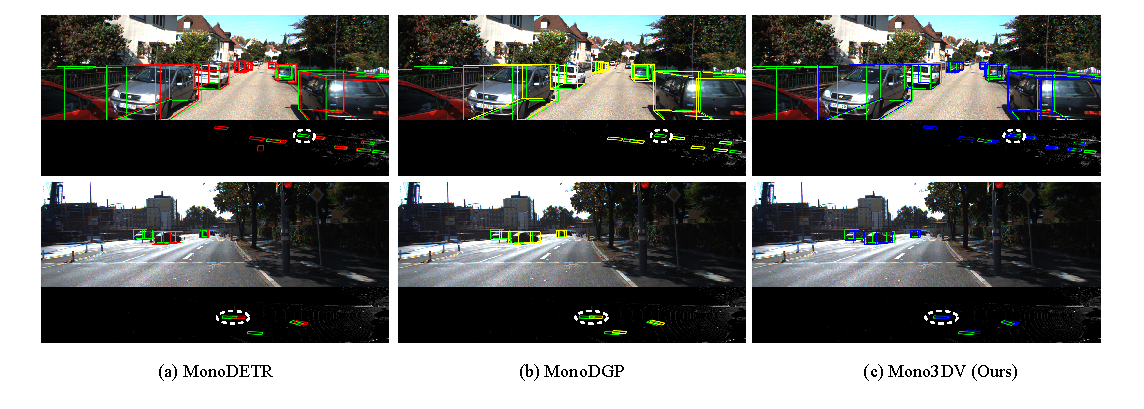
\includegraphics[width=\textwidth]{images/mono3dv/qualitative_results.pdf}
    \caption{\textbf{Qualitative results on KITTI val set.} (a) MonoDETR~\cite{MonoDETR}. (b) MonoDGP~\cite{MonoDGP}. (c) Mono3DV (Ours). For each image set, the top row presents the camera-view visualization, while the bottom row offers the corresponding bird’s-eye view. Ground-truth bounding boxes are rendered in \textcolor{green}{green}, and predictions are shown in order: \textcolor{red}{red}, \textcolor{yellow}{yellow}, \textcolor{blue}{blue}. We also circle some objects to highlight the difference between other state-of-the-art methods and our method.}
\label{fig:qualitative_results}
\end{figure*}